\chapter{映射}
\section{连续映射}

\begin{definition}{连续映射}
    设$X,Y$是拓扑空间，$f:X\to Y$是一个映射. 如果对$Y$中任意开集$V$，其原像$f^{-1}(V)$在$X$中是开集，则称$f$是\textbf{连续的}.
\end{definition}

\begin{instance}
    \begin{enumerate}
        \item 恒等映射 $\setjot[-10]\begin{aligned}[t]
            \mathrm{id}:X &\to X \\ 
            x &\mapsto x
        \end{aligned}$ 是连续的.
        \item 常值映射 $\setjot[-10]\begin{aligned}[t]
            c:X&\to Y \\ 
            x&\mapsto y_0
        \end{aligned}$ 是连续的.
        \item $X$是拓扑空间，$A\subset X$，则包含映射 $\setjot[-10]\begin{aligned}[t]
            i:A &\to X \\ 
            x&\mapsto x
        \end{aligned}$ (其中$A$是$X$的子空间) 是连续的.
        \item $X,Y$是拓扑空间，在乘积空间$X\times Y$上投射 $\setjot[-10]\begin{aligned}[t]
            \pi_1:X\times Y &\to X \\ 
            (x,y)&\mapsto x
        \end{aligned}$ 和 $\setjot[-10]\begin{aligned}[t]
            \pi_2:X\times Y &\to Y \\ 
            (x,y)&\mapsto y
        \end{aligned}$ 是连续的.
    \end{enumerate}
\end{instance}

\begin{lemma}
    若$f:X\to Y$和$g:Y\to Z$是连续映射，则复合映射$g\circ f:X\to Z$也是连续的.
\end{lemma}
\begin{proof}
    $\forall\,\open V\in Z$，$(g\circ f)^{-1}(V)=f^{-1}(g^{-1}(V))$.\par 
    因为$g$连续，$g^{-1}(V)$是$Y$中的开集.又因为$f$连续，$f^{-1}(g^{-1}(V))$是$X$中的开集.
\end{proof}

\begin{instance}
    $f:X\to Y$是连续映射，$A\subset X$，则$f|_A：A\to Y$是连续的.\par
        \begin{wrapfigure}{r}{0.25\textwidth}
        \vspace{-2.8 em}
        \begin{tikzcd}[column sep=2.4em, row sep=1.8em,every label/.append style={font=\normalsize},font=\normalsize]
            A \arrow[rr, "f|_A"] \arrow[rd, "i"'] &                    & Y \\
                                      & X \arrow[ru, "f"'] &  
        \end{tikzcd}
        \vspace{-2 em}
    \end{wrapfigure}
    回顾之前的内容，限制映射有如右图所示的交换图，即$f|_A=f\circ i$.\par
    又$f$和$i$都是连续的，因此$f|_A$也是连续的.
\end{instance}

\begin{lemma}
    设$f:X\to Y$是一个映射，$\mcal{B}$是$Y$的一个拓扑基，则$f$是连续的$\Leftrightarrow \forall\, B\in\mcal{B},f^{-1}(B)$是$X$中的开集.
\end{lemma}
这个定理的证明只需要利用连续映射的定义和拓扑基生成拓扑的方式即可完成.\par
这一引理让我们不必讨论$Y$中所有开集的原像，只需讨论基元素的原像.\par

\begin{instance}
    (1)\; $\setjot[-10]\begin{aligned}[t]
        f: \mb{E}^1 &\to \mb{E}^1 \\
        x &\mapsto f(x)=x^n,e^x,\ln{x},\sin{x},\cos{x}
    \end{aligned}$都是连续函数.\par
    (2)\; $\setjot[-10]\begin{aligned}[t]
        f:\mb{E}^2 &\to \mb{E}^1 \\
        (x,y) &\mapsto f(x,y)=x+y,x-y,xy,\frac{x}{y}(y\neq 0)
    \end{aligned}$都是连续函数.
\end{instance}

\begin{lemma}
    $f:X\to Y$是一个映射，则$f$是连续的$\Leftrightarrow \forall\,\close C\in Y,f^{-1}(C)$是$X$中的闭集.
\end{lemma}
这个引理相较于连续映射最初始的定义，只是将其中的开集改为闭集.成立的原因是开集取补就是闭集.\par

\begin{proposition}
    设$f:X\to Y_1\times Y_2$是一个映射，定义为$f(x)=(f_1(x),f_2(x))$，其中$f_1:X\to Y_1, f_2:X\to Y_2$. 则$f$连续$\Leftrightarrow f_1$和$f_2$都连续.
\end{proposition}
\begin{proof}
    “$\Rightarrow$” 投射$\setjot[-10]\begin{aligned}[t]
            \pi_1:X\times Y &\to X \\ 
            (x,y)&\mapsto x
        \end{aligned}$ 和 $\setjot[-10]\begin{aligned}[t]
            \pi_2:X\times Y &\to Y \\ 
            (x,y)&\mapsto y
        \end{aligned}$都是连续的.\par
    $f_1=\pi_1\circ f, f_2=\pi_2\circ f$. 由于投射和$f$是连续的，所以$f_1,f_2$都连续.\par
    “$\Leftarrow$” $\mcal{B}=\{U_1\times U_2|U_i\text{是}Y_i\text{中的开集}\}$是$Y_1\times Y_2$的一个拓扑基.\par
    $f^{-1}(U_1\times U_2)= f_1^{-1}(U_1)\cap f_2^{-1}(U_2)$. 由于$f_1,f_2$连续，$f_1^{-1}(U_1)$和$f_2^{-1}(U_2)$都是$X$中的开集.\par
    因此$f^{-1}(U_1\times U_2)$是$X$中的开集.
\end{proof}

\begin{lemma}{引理 (Pasting Lemma)}
    $X$是一个拓扑空间，$A,B$是$X$中的闭集且$X=A\cup B$.设$f:A\to Y$和$g:B\to Y$是两个连续映射，且对任意$x\in A\cap B$都有$f(x)=g(x)$. 则由它们定义的映射
    \[h:X\to Y, x\mapsto\begin{cases} f(x) & x\in A \\ g(x) & x\in B \end{cases}\]
    是连续的.
\end{lemma}
\begin{figure}[h]
    \centering
    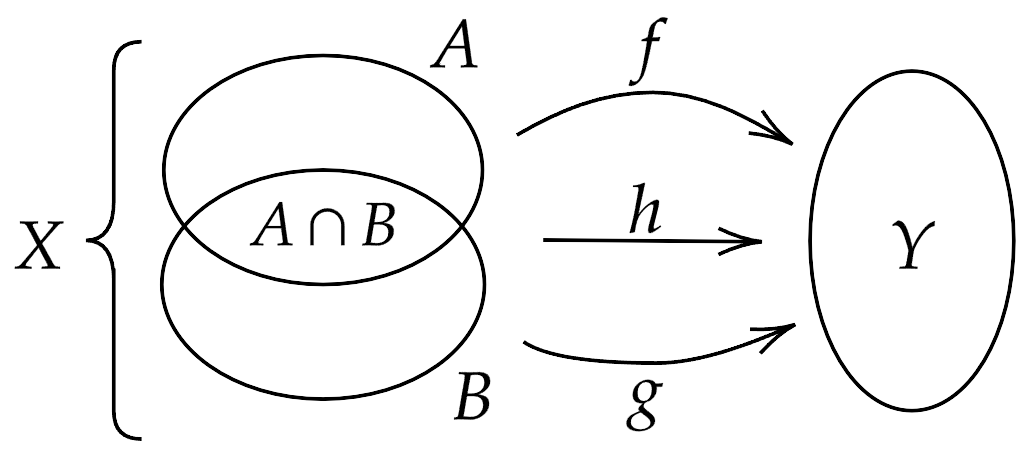
\includegraphics[width=0.4\textwidth]{fig/2.12.png}
    \captionof{figure}{粘贴引理示意图}
\end{figure}
\begin{proof}
    $\forall\,\close C\in Y$，则$f^{-1}(C)$是$A$中的闭集，$g^{-1}(C)$是$B$中的闭集，且$h^{-1}(C)=f^{-1}(C)\cup g^{-1}(C)$.\par
    根据定义，$\exists\,\close D_1\in X,\st f^{-1}(C)=D_1\cap A$.\par
    同理，$\exists\,\close D_2\in X,\st g^{-1}(C)=D_2\cap B$.\par
    因为$A,B$都是$X$中的闭集，$f^{-1}(C)$和$g^{-1}(C)$都是$X$中的闭集，因此$h^{-1}(C)=f^{-1}(C)\cup g^{-1}(C)$也是$X$中的闭集.
\end{proof}